\section{Exercícios}

\subsection{Análise Nodal}

Relativo a análise nodal serão feitos os problemas: 3.2, 3.3, 3.5, 3.7, 3.8,
3.9, 3.10, 3.12, 3.14, 3.17, 3.18, 3.19, 3.20, 3.22, 3.24, 3.25, 3.26, 3.28,
3.30, 3.31, 3.32. Nesta ordem.

\question{Para o circuito da Figura~\ref{fig:fig3.2}, obtenha $v_1$ e $v_2$.}
\begin{figure}[H]
  \centering
  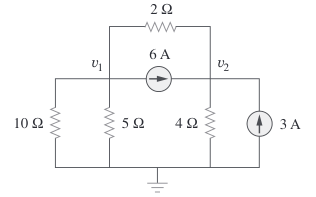
\includegraphics[width=0.5\textwidth]{./fig/fig3.2.png}
  \caption{Esquema para o Problema 1}\label{fig:fig3.2}
\end{figure}
\answer{
  \begin{align*}
    &\text{Para } v_1: \\
    &\frac{v_1 - 0}{10} + \frac{v_1 - 0}{5} + 6 + \frac{v_1 - v_2}{2} = 0 \\
    &\frac{v_1}{10} + \frac{v_1}{5} + \frac{v_1 - v_2}{2} + 6 = 0 \\[8pt]
    &\text{Para } v_2: \\
    &-6 + \frac{v_2 - v_1}{2} + \frac{v_2 - 0}{4} - 3 = 0 \\
    &\frac{v_2 - v_1}{2} + \frac{v_2}{4} - 9 = 0 \\[8pt]
    &\begin{cases}
      \dfrac{v_1}{10} + \dfrac{v_1}{5} + \dfrac{v_1 - v_2}{2} + 6 = 0 \\[8pt]
      \dfrac{v_2 - v_1}{2} + \dfrac{v_2}{4} - 9 = 0 \\
    \end{cases}\\[8pt]
    &v_1 = \boxed{-3\,\text{V}} \\
    &v_2 = \boxed{10\,\text{V}}
  \end{align*}
}

\question{Determine as correntes $I_1$ a $I_4$ e a tensão $v_0$ no circuito da
Figura~\ref{fig:fig3.3}.}
\begin{figure}[H]
  \centering
  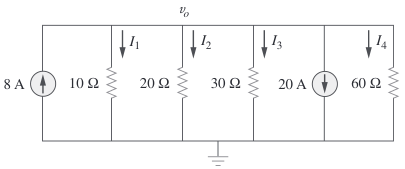
\includegraphics[width=0.5\textwidth]{./fig/fig3.3.png}
  \caption{Esquema para o Problema 2}\label{fig:fig3.3}
\end{figure}
\answer{
  \begin{align*}
    &\text{Resistência Equivalente (} Req \text{):} \\
    &\frac{1}{Req} = \frac{1}{10} + \frac{1}{20} + \frac{1}{30} + \frac{1}{60} \\
    &\frac{1}{Req} = \frac{6 + 3 + 2 + 1}{60} \\
    &\frac{1}{Req} = \frac{12}{60} \\
    &Req = \frac{60}{12} \\
    &Req = 5 \Omega \\[8pt]
    &\text{Corrente Total (} I_t \text{):} \\
    &I_t = 8 - 20 \\
    &I_t = -12 A \\[8pt]
    &v_0\text{:} \\
    &v_0 = I_t \cdot Req \\
    &v_0 = -12 \cdot 5 \\
    &v_0 = \boxed{-60V} \\[8pt]
    &I_1 \ldots I_4\text{:} \\
    &I = \frac{R}{V} \\
    &\begin{cases}
      I_1 = \frac{-60}{10} = \boxed{-6A} \\
      I_2 = \frac{-60}{20} = \boxed{-3A} \\
      I_3 = \frac{-60}{30} = \boxed{-2A} \\
      I_4 = \frac{-60}{-60} = \boxed{1A} \\
    \end{cases}
  \end{align*}
}

\newpage
\question{Obtenha $v_0$ no circuito da Figura~\ref{fig:fig3.5}.}
\begin{figure}[H]
  \centering
  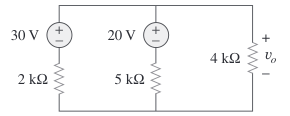
\includegraphics[width=0.5\textwidth]{./fig/fig3.5.png}
  \caption{Esquema para o Problema 3}\label{fig:fig3.5}
\end{figure}
\answer{
  \begin{align*}
    &\text{Definindo nós:} \\
    &\textit{Nó 1:} \, \text{Entre a fonte de 30V, o resistor de 2k}\Omega\text{ e o resistor de 4k}\Omega\text{.}\\
    &\textit{Nó 2:} \, \text{Entre a fonte de 20V, o resistor de 5k}\Omega\text{ e o resistor de 4k}\Omega\text{.} \\[8pt]
    &v_1\text{:} \\
    &\frac{30 - v_1}{2} = \frac{v_1}{4} + \frac{v_1 - 20}{5} \\
    &v_1 = \frac{380}{19} \\
    &v_1 = 20V \\[8pt]
    &v_2\text{:} \\
    &\frac{20 - v_2}{5} + \frac{20 - v_2}{4} = 0 \\
    &v_2 = \frac{180}{9} \\
    &v_2 = 20V \\[8pt]
    &v_0 = v_2 = \boxed{20V} \\
  \end{align*}
}

\newpage
\question{Aplique a análise nodal para determinar $V_x$ no circuito da
Figura~\ref{fig:fig3.7}.}
\begin{figure}[H]
  \centering
  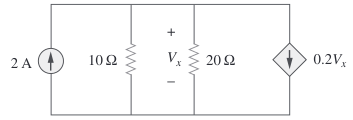
\includegraphics[width=0.5\textwidth]{./fig/fig3.7.png}
  \caption{Esquema para o Problema 4}\label{fig:fig3.7}
\end{figure}
\answer{
  \begin{align*}
    &LKC\text{:} \\
    &\frac{V_x}{10} + \frac{V_x}{20} + 0.2V_x = 2\\
    &2V_x + V_x + 4V_x = 40\\
    &7V_x = 40\\
    &V_x = \frac{40}{7} = \boxed{5.714} \\
  \end{align*}
}

\newpage
\question{Usando análise nodal, determine $v_0$ no circuito da
Figura~\ref{fig:fig3.8}.}
\begin{figure}[H]
  \centering
  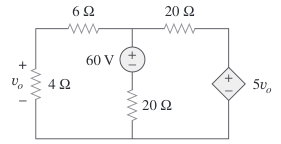
\includegraphics[width=0.5\textwidth]{./fig/fig3.8.png}
  \caption{Esquema para o Problema 5}\label{fig:fig3.8}
\end{figure}
\answer{
  \begin{align*}
    &v_2 = 5v_0 \\[8pt]
    &v_0\text{:} \\
    &\frac{v_0 - 0}{4} + \frac{v_0 - v_1}{6} = 0 \\
    &3v_0 + 2v_0 - 2v_1 = 0 \\
    &5v_0 - 2v_1 = 0 \\
    &v_0 = \frac{2v_1}{5} \\[8pt]
    &v_1\text{:} \\
    &\frac{v_1 - v_0}{6} + \frac{v_1 - 60}{20} + \frac{v_1 - 5v_0}{20} = 0 \\
    &10v_1 - 10v_0 + 3v_1 - 180 + 3v_1 - 15v_0 = 0 \\
    &16v_1 - 25v_0 = 180 \\
    &16v_1 - 25(\frac{2v_1}{5}) = 180 \\
    &16v_1 - 5v_1 = 180 \\
    &11v_1 = 180 \\
    &v_1 = \frac{180}{11} = \boxed{16.36V} \\
    &v_0 = \frac{2(\frac{180}{11})}{5} \\
    &v_0 = \frac{72}{11} = \boxed{6.55V} \\
    &v_2 = 5(\frac{72}{11}) = \boxed{32.73V} \\
  \end{align*}
}

\newpage
\question{Determine $I_b$ no circuito da Figura~\ref{fig:fig3.9}, usando análise
nodal.}
\begin{figure}[H]
  \centering
  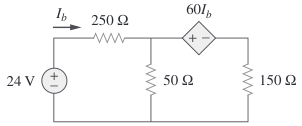
\includegraphics[width=0.5\textwidth]{./fig/fig3.9.png}
  \caption{Esquema para o Problema 6}\label{fig:fig3.9}
\end{figure}
\answer{
  \begin{align*}
    &I_b = \frac{24 - v_1}{250} \\[8pt]
    &v_1\text{:} \\
    &\frac{24 - v_1}{250} = \frac{v_1 - 0}{50} + \frac{v_1 - 60I_b}{150} \\
    &15(24 - v_1) = 75v_1 + 25(v_1 - 60I_b) \\
    &360 - 15v_1 = 75v_1 + 25v_1 - 1500I_b \\
    &360 - 150v_1 = -1500(\frac{24 - v_1}{250}) \\
    &360 - 150v_1 = -144 + 6v_1 \\
    &360 + 144 = 150v_1 + 6v_1 \\
    &156v_1 = 504 \\
    &v_1 = \frac{504}{156} = \frac{42}{13} = 3.23077V \\[8pt]
    &I_b = \frac{24 - \frac{42}{13}}{250} = \frac{27}{325} = 0.08307A = \boxed{83.07mA} \\
  \end{align*}
}

\question{Determine $I_0$ no circuito da Figura~\ref{fig:fig3.10}.}
\begin{figure}[H]
  \centering
  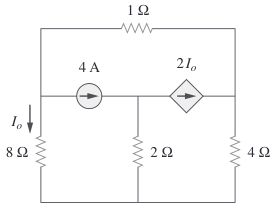
\includegraphics[width=0.5\textwidth]{./fig/fig3.10.png}
  \caption{Esquema para o Problema 7}\label{fig:fig3.10}
\end{figure}
\answer{
  \begin{align*}
    &I_0 = \frac{v_1}{8} \\[8pt]
    &v_1\text{:} \\
    &\frac{v_1 - 0}{8} + 4 + \frac{v_1 - v_3}{1} = 0 \\
    &v_1 + 32 + 8v_1 - 8v_3 = 0 \\
    &9v_1 - 8v_3 = -32 \\[8pt]
    &v_2\text{:} \\
    &\frac{v_2 - 0}{2} + 2I_0 = 4 \\
    &\frac{v_2}{2} + 2\frac{v_1}{8} = 4 \\
    &\frac{v_2}{2} + \frac{v_1}{4} = 4 \\
    &2v_2 + v_1 = 16 \\
    &v_1 + 2v_2 = 16 \\[8pt]
    &v_3\text{:} \\
    &2I_0 + \frac{v_3 - v_1}{1} = \frac{v_3 - 0}{4}  \\
    &2\frac{v_1}{8} + v_3 - v_1 = \frac{v_3}{4}  \\
    &\frac{v_1}{4} + v_3 - v_1 = \frac{v_3}{4}  \\
    &v_1 + 4v_3 - 4v_1 = v_3  \\
    &-3v_1 + 3v_3= 0  \\
    &1v_1 - 1v_3= 0  \\[8pt]
    &\begin{cases}
      9v_1 - 8v_3 = -32 \\
      v_1 + 2v_2 = 16 \\
      v_1 - v_3= 0  \\
    \end{cases}\\
    &v_1 = v_3 = -32V \\
    &v_2 = 24V \\
    &I_0 = \frac{-32}{8} = \boxed{-4} \\
  \end{align*}
}

\newpage
\question{Usando análise nodal, determine $V_0$ no circuito da
Figura~\ref{fig:fig3.12}.}
\begin{figure}[H]
  \centering
  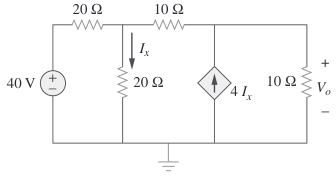
\includegraphics[width=0.5\textwidth]{./fig/fig3.12.png}
  \caption{Esquema para o Problema 8}\label{fig:fig3.12}
\end{figure}
\answer{
  \begin{align*}
    &I_x = \frac{v_2}{20} \\
    &v_1 = 40V \\[8pt]
    &v_3\text{:} \\
    &4I_x + \frac{v_2 - v_3}{10} = \frac{v_3 - 0}{10} \\
    &40I_x + v_2 - v_3 = v_3 \\
    &40\frac{v_2}{20} + v_2 - 2v_3 = 0 \\
    &3v_2 - 2v_3 = 0 \\
    &3v_2 = 2v_3 \\
    &v_2 = \frac{2v_3}{3} \\[8pt]
    &v_2\text{:} \\
    &\frac{40 - v_2}{20} = \frac{v_2 - 0}{20} + \frac{v_2 - v_3}{10} \\
    &40 - v_2 = v_2 + 2v_2 - 2v_3 \\
    &4v_2 - 2v_3 = 40 \\[8pt]
    &4(\frac{2v_3}{3}) - 2v_3 = 40 \\
    &\frac{2v_3}{3} = 40 \\
    &2v_3 = 120 \\
    &v_3 = \frac{120}{2} = 60V \\
    &v_2 = \frac{2 \cdot 60}{3} = \frac{120}{3} = 40V \\
    &v_0 = v_3 = \boxed{60V} \\
  \end{align*}
}

\newpage
\question{Usando análise nodal, determine $v_0$ no circuito da
Figura~\ref{fig:fig3.14}.}
\begin{figure}[H]
  \centering
  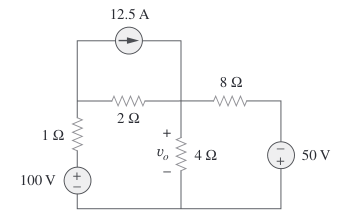
\includegraphics[width=0.5\textwidth]{./fig/fig3.14.png}
  \caption{Esquema para o Problema 9}\label{fig:fig3.14}
\end{figure}
\answer{
  \begin{align*}
    &v_0 = v_2 \\
    &v_3 = -50 \\[8pt]
    &v_2\text{:} \\
    &12.5 + \frac{v_1 - v_2}{2} = \frac{v_2 - 0}{4} + \frac{v_2 - v_3}{8} \\
    &100 + 4v_1 - 4v_2 = 2v_2 + v_2 - v_3 \\
    &7v_2 - v_3 - 4v_1 = 100 \\
    &7v_2 + 50 - 4v_1 = 100 \\
    &7v_2 - 4v_1 = 50 \\[8pt]
    &v_1\text{:} \\
    &\frac{100 - v_1}{1} = \frac{v_1 - v_2}{2} + 12.5 \\
    &200 - 2v_1 = v_1 - v_2 + 25 \\
    &3v_1 - v_2 = 175 \\[8pt]
    &\begin{cases}
      &-4v_1 + 7v_2 = 50 \\
      &3v_1 - v_2 = 175 \\
    \end{cases}\\
    &v_1 = 75V \\
    &v_2 = 50V \\
    &v_0 = v_2 = \boxed{50V} \\
  \end{align*}
}

\newpage
\question{Usando análise nodal, determine a corrente $i_0$ no circuito da
Figura~\ref{fig:fig3.17}.}
\begin{figure}[H]
  \centering
  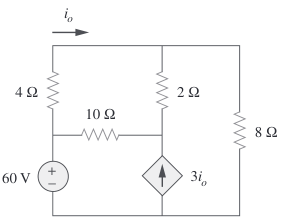
\includegraphics[width=0.5\textwidth]{./fig/fig3.17.png}
  \caption{Esquema para o Problema 10}\label{fig:fig3.17}
\end{figure}
\answer{
  \begin{align*}
    &v_1 = 60V \\
    &i_0 = \frac{60 - v_3}{4} \\[8pt]
    &v_3\text{:} \\
    &\frac{60 - v_3}{4} = \frac{v_3 - v_2}{2} + \frac{v_3 - 0}{8} \\
    &120 - 2v_3 = 4v_3 - 4v_2 + v_3 \\
    &-4v_2 + 7v_3 = 120\\[8pt]
    &v_2\text{:} \\
    &\frac{60 - v_2}{10} + \frac{v_3 - v_2}{2} + 3i_0 = 0 \\
    &\frac{60 - v_2}{10} + \frac{v_3 - v_2}{2} + 15i_0 = 0 \\
    &\frac{60 - v_2}{10} + \frac{v_3 - v_2}{2} + \frac{900 - 15v_3}{4} = 0 \\
    &120 - 2v_2 + 10v_3 - 10v_2 + 900 - 15v_3 = 0 \\
    &5v_2 + 12v_3 = 1020 \\[8pt]
    &\begin{cases}
      &-4v_2 + 7v_3 = 120\\
      &5v_2 + 12v_3 = 1020 \\
    \end{cases}\\
    &v_2 = \frac{5700}{83} = 68.67V\\
    &v_3 = \frac{4680}{83} = 56.39V\\
    &i_0 = \frac{60 - \frac{4680}{83}}{4} = \frac{75}{83} = \boxed{0.90A} \\
  \end{align*}
}

\newpage
\question{Determine as tensões nodais no circuito da Figura~\ref{fig:fig3.18}
usando análise nodal.}
\begin{figure}[H]
  \centering
  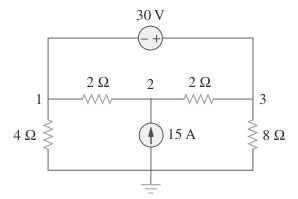
\includegraphics[width=0.5\textwidth]{./fig/fig3.18.png}
  \caption{Esquema para o Problema 11}\label{fig:fig3.18}
\end{figure}
\answer{
  \begin{align*}
    &v_3\text{:} \\
    &i_3 + \frac{v_2 - v_3}{2} = \frac{v_3 - 0}{8} \\
    &i_3 = \frac{v_3 - 0}{8} - \frac{v_2 - v_3}{2} \\[8pt]
    &v_1\text{:} \\
    &\frac{v_2 - v_1}{2} = \frac{v_1 - 0}{4} + \frac{v_3}{8} - \frac{v_2 - v_3}{2} \\
    &4v_2 - 4v_1 = 2v_1 + v_3 - 4v_2 + 4v_3 \\
    &4v_2 - 4v_1 = 2v_1 - 4v_2 + 5v_3 \\
    &6v_1 - 8v_2 - 5v_3 = 0\\[8pt]
    &v_3 - v_1 = 30 \\
    &v_3  = 30 + v_1 \\[8pt]
    &6v_1 - 8v_2 - 5(30 + v_1) = 0\\
    &6v_1 - 8v_2 - 150 + 5v_1 = 0\\
    &11v_1 - 8v_2 = 150\\[8pt]
    &v_2\text{:} \\
    &15 = \frac{v_2 - v_1}{2} + \frac{v_2 - v_3}{2} \\
    &30 = v_2 - v_1 + v_2 - v_3 \\
    &30 = v_2 - v_1 + v_2 - 30 + v_1 \\
    &30 = 2v_2 - 30 \\[8pt]
    &v_1 = \boxed{30V} \\
    &v_2 = \boxed{60V} \\
    &v_3 = \boxed{60V} \\
  \end{align*}
}

\newpage
\question{Use a análise nodal para determinar $v_1$, $v_2$ e $v_3$ no circuito
da Figura~\ref{fig:fig3.19}.}
\begin{figure}[H]
  \centering
  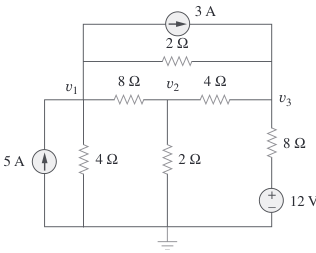
\includegraphics[width=0.5\textwidth]{./fig/fig3.19.png}
  \caption{Esquema para o Problema 12}\label{fig:fig3.19}
\end{figure}
\answer{
  \begin{align*}
    &v_1\text{:} \\
    &3 + \frac{v_1 - v_3}{2} + \frac{v_1 - v_2}{8} + \frac{v_1 - 0}{4} = 5 \\
    &\frac{v_1 - v_3}{2} + \frac{v_1 - v_2}{8} + \frac{v_1 - 0}{4} = 2 \\
    &4v_1 - 4v_3 + v_1 - v_2 + 2v_1 = 16 \\
    &7v_1 - v_2 - 4v_3 = 16 \\[8pt]
    &v_2\text{:} \\
    &\frac{v_1 - v_2}{8} = \frac{v_2 - 0}{2} + \frac{v_2 - v_3}{4} \\
    &v_1 - v_2 = 4v_2 + 2v_2 - 2v_3 \\
    &-v_1 + 9v_2 - 2v_3 = 0 \\[8pt]
    &v_3\text{:} \\
    &\frac{v_2 - v_3}{4} + \frac{v_1 - v_3}{2} + 3 = \frac{v_3 - 12}{8} \\
    &2v_2 - 2v_3 + 4v_1 - 4v_3 + 24 = v_3 - 12 \\
    &4v_1 + 2v_2 - 7v_3 = -36 \\[8pt]
    &\begin{cases}
      &7v_1 - v_2 - 4v_3 = 16 \\
      &-v_1 + 9v_2 - 2v_3 = 0 \\
      &4v_1 + 2v_2 - 7v_3 = -36 \\
    \end{cases}\\
    &v_1 = \boxed{10V} \\
    &v_2 = \boxed{4.933V} \\
    &v_3 = \boxed{12.267V} \\
  \end{align*}
}

\newpage
\question{Para o circuito da Figura~\ref{fig:fig3.20}, determine $v_1$ e $v_2$
usando análise nodal.}
\begin{figure}[H]
  \centering
  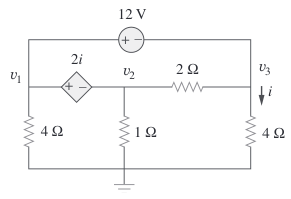
\includegraphics[width=0.5\textwidth]{./fig/fig3.20.png}
  \caption{Esquema para o Problema 13}\label{fig:fig3.20}
\end{figure}
\answer{
  \begin{align*}
    &i = \frac{v_3}{4} \\[8pt]
    &i_2\text{:} \\
    &i_2 = \frac{v_2}{1} + \frac{v_2 - v_3}{2} \\[8pt]
    &i_3\text{:} \\
    &i_3 = \frac{v_3}{4} - \frac{v_2 - v_3}{2} \\[8pt]
    &v_1\text{:} \\
    &\frac{v_1 - 0}{4} + i_2 + i_3 = 0 \\
    &v_1 + 4v_2 - 3v_3 = 0 \\[8pt]
    &v_3\text{:} \\
    &v_1 - v_3 = 12 \\
    &v_3 = v_1 - 12 \\[8pt]
    &v_2\text{:} \\
    &v_1 - v_2 = 2i \\
    &v_1 - v_2 = 2\frac{v_3}{4} \\
    &v_1 - v_2 = \frac{v_3}{2} \\
    &2v_1 - 2v_2 - v_3 = 0 \\[8pt]
    &\begin{cases}
      &v_1 + 2v_2 = 6 \\
      &v_1 - 2v_2 = -12 \\
    \end{cases}\\
    &v_1 = \boxed{-3V} \\
    &v_2 = \boxed{4.5V} \\
    &v_3 = \boxed{-15V} \\
  \end{align*}
}

\newpage
\question{Determine $v_1$ e $v_2$ para o circuito da Figura~\ref{fig:fig3.22}.}
\begin{figure}[H]
  \centering
  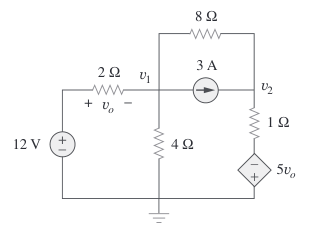
\includegraphics[width=0.5\textwidth]{./fig/fig3.22.png}
  \caption{Esquema para o Problema 14}\label{fig:fig3.22}
\end{figure}
\answer{
  \begin{align*}
    &v_A = 12 \\
    &v_0 = 12 - v_1 \\[8pt]
    &v_1\text{:} \\
    &\frac{12 - v_1}{2} = \frac{v_1 - 0}{4} + \frac{v_1 - v_2}{8} + 3 \\
    &48 - 4v_1 = 2v_1 + v_1 - v_2 + 24 \\
    &7v_1 - v_2 = 24 \\[8pt]
    &v_2\text{:} \\
    &3 + \frac{v_1 - v_2}{8} = \frac{v_2 - 5v_0}{1} \\
    &24 + v_1 - v_2 = 8v_2 + 40v_0 \\
    &24 + v_1 - v_2 = 8v_2 + 40(12 - v_1) \\
    &24 + v_1 - v_2 = 8v_2 + 480 - 40v_1 \\
    &41v_1 - 9v_2 = 456 \\[8pt]
    &\begin{cases}
      &7v_1 - v_2 = 24 \\
      &41v_1 - 9v_2 = 456 \\
    \end{cases}\\
    &v_1 = -\frac{240}{22} = \boxed{-10.909V} \\
    &v_2 = \boxed{-100.363V} \\
  \end{align*}
}

\newpage
\question{Use a análise nodal e o \textit{MATLAB} para determinar $V_0$ no
circuito da Figura~\ref{fig:fig3.24}.}
\begin{figure}[H]
  \centering
  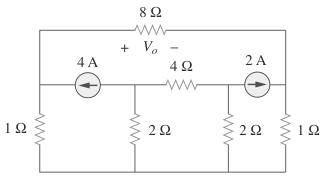
\includegraphics[width=0.5\textwidth]{./fig/fig3.24.png}
  \caption{Esquema para o Problema 15}\label{fig:fig3.24}
\end{figure}
\answer{
  \begin{align*}
    &v_1\text{:} \\
    &4 = \frac{V_1}{1} + \frac{V_1 - V_4}{8} \\
    &32 = 8V_1 + V_1 - V_4 \\
    &32 = 9V_1 - V_4 \\[8pt]
    &v_4\text{:} \\
    &2 + \frac{V_1 - V_4}{8} = \frac{V_4}{1} \\
    &16 + V_1 - V_4 = 8V_4 \\
    &1V_1 - 9V_4 = -16 \\[8pt]
    &\begin{cases}
      &9V_1 - V_4 = 32\\
      &1V_1 - 9V_4 = -16 \\
    \end{cases}\\
    &v_1 = 3.8V \\
    &v_2 = 2.2V \\
    &v_0 = v_1 - v_2 = \boxed{1.6V} \\
  \end{align*}
}

\newpage
\question{Use análise nodal juntamente com o \textit{MATLAB} para determinar as
tensões nos nós da Figura~\ref{fig:fig3.25}.}
\begin{figure}[H]
  \centering
  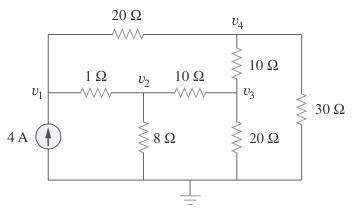
\includegraphics[width=0.5\textwidth]{./fig/fig3.25.png}
  \caption{Esquema para o Problema 16}\label{fig:fig3.25}
\end{figure}
\answer{
  \begin{align*}
    &v_1\text{:} \\
    &4 = \frac{v_1 - v_2}{1} + \frac{v_1 - v_4}{20} \\
    &80 = 20v_1 - 20v_2 + v_1 - v_4 \\
    &80 = 21v_1 - 20v_2 - v_4 \\[8pt]
    &v_2\text{:} \\
    &\frac{v_1 - v_2}{1} = \frac{v_2}{8} + \frac{v_2 - v_3}{10} \\
    &40v_1 - 40v_2 = 5v_2 + 4v_2 - 4v_3 \\
    &40v_1 - 49v_2 + 4v_3 = 0 \\[8pt]
    &v_3\text{:} \\
    &\frac{v_2 - v_3}{10} + \frac{v_4 - v_3}{10} = \frac{v_3}{20} \\
    &2v_2 - 2v_3 + 2v_4 - 2v_3 = v_3 \\
    &2v_2 - 5v_3 + 2v_4 = 0 \\[8pt]
    &v_4\text{:} \\
    &\frac{v_1 - v_4}{20} = \frac{v_4 - v_3}{10} + \frac{v_4}{30} \\
    &3v_1 - 3v_4 = 6v_4 - 6v_3 + 2v_4 \\
    &3v_1 + 6v_3 - 11v_4 = 0  \\[8pt]
    &\begin{cases}
      &21v_1 - 20v_2 - v_4 = 80\\
      &40v_1 - 49v_2 + 4v_3 = 0 \\
      &2v_2 - 5v_3 + 2v_4 = 0 \\
      &3v_1 + 6v_3 - 11v_4 = 0  \\
    \end{cases}\\
    &v_1 = \boxed{25.52V} \\
    &v_2 = \boxed{22.05V} \\
    &v_3 = \boxed{14.84V} \\
    &v_4 = \boxed{15.06V} \\
  \end{align*}
}

\newpage
\question{Calcule as tensões nodais $v_1$, $v_2$ e $v_3$ no circuito da
Figura~\ref{fig:fig3.26}.}
\begin{figure}[H]
  \centering
  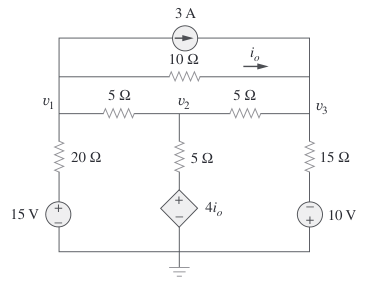
\includegraphics[width=0.5\textwidth]{./fig/fig3.26.png}
  \caption{Esquema para o Problema 17}\label{fig:fig3.26}
\end{figure}
\answer{
  \begin{align*}
    &v_1\text{:} \\
    &\frac{v_1 - 15}{20} + \frac{v_1 - v_2}{5} + 3 + \frac{v_1 - v_3}{10} = 0 \\
    &v_1 - 15 + 4v_1 - 4v_2 + 60 + 2v_1 - 2v_3 = 0 \\
    &7v_1 - 4v_2 - 2v_3 = -45 \\[8pt]
    &v_2\text{:} \\
    &\frac{v_1 - v_2}{5} = \frac{v2 - 4i_0}{5} + \frac{v_2 - v_3}{5} \\
    &v_1 - v_2 = v2 - 4i_0 + v_2 - v_3 \\
    &v_1 - 3v_2 + v_3 + 4i_0 = 0 \\
    &v_1 - 3v_2 + v_3 + 4\frac{v_1 - v_3}{10} = 0 \\
    &10v_1 - 30v_2 + 10v_3 + 4v_1 - 4v_3 = 0 \\
    &14v_1 - 30v_2 + 6v_3 = 0 \\[8pt]
    &v_3\text{:} \\
    &\frac{v_1 - v_3}{10} + 3 + \frac{v_2 - v_3}{5} = \frac{v_3 + 10}{15} \\
    &3v_1 - 3v_3 + 90 + 6v_2 - 6v_3 = 2v_3 + 20 \\
    &3v_1 + 6v_2 - 11v_3 = - 70 \\[8pt]
    &\begin{cases}
      &7v_1 - 4v_2 - 2v_3 = -45 \\
      &14v_1 - 30v_2 + 6v_3 = 0 \\
      &3v_1 + 6v_2 - 11v_3 = - 70 \\
    \end{cases}\\
    &v_1 = \boxed{-7.1918V} \\
    &v_2 = \boxed{-2.7789V} \\
    &v_3 = \boxed{2.8865V} \\
  \end{align*}
}

\newpage
\question{Use o \textit{MATLAB} para determinar as tensões nos nós $a$, $b$, $c$
e $d$ no circuito da Figura~\ref{fig:fig3.28}.}
\begin{figure}[H]
  \centering
  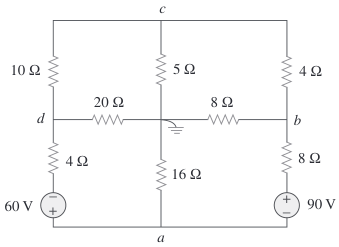
\includegraphics[width=0.4\textwidth]{./fig/fig3.28.png}
  \caption{Esquema para o Problema 18}\label{fig:fig3.28}
\end{figure}
\answer{
  \begin{align*}
    &v_a\text{:} \\
    &0 = \frac{v_a - 60 - v_d}{4} + \frac{v_a}{16} + \frac{v_a + 90 - v_b}{8} \\
    &0 = 4v_a - 240 - 4v_d + v_a + 2v_a + 180 - 2v_b \\
    &7v_a - 2v_b - 4v_d = 60 \\[8pt]
    &v_b\text{:} \\
    &\frac{v_a + 90 - v_b}{8} = \frac{v_b}{8} + \frac{v_b - v_c}{4} \\
    &v_a + 90 - v_b = v_b + 2v_b - 2v_c \\
    &v_a - 4v_b + 2v_c = -90 \\[8pt]
    &v_c\text{:} \\
    &\frac{v_d - v_c}{10} + \frac{v_b - v_c}{4} = \frac{v_c}{5} \\
    &2v_d - 2v_c + 5v_b - 5v_c = 4v_c \\
    &5v_b - 11v_c + 2v_d = 0 \\[8pt]
    &v_d\text{:} \\
    &\frac{v_a - 60 - v_d}{4} = \frac{v_d}{20} + \frac{v_d - v_c}{10} \\
    &5v_a - 300 - 5v_d = v_d + 2v_d - 2v_c \\
    &5v_a + 2v_c - 8v_d = 300 \\[8pt]
    &\begin{cases}
      &7v_a - 2v_b - 4v_d = 60 \\
      &v_a - 4v_b + 2v_c = -90 \\
      &5v_b - 11v_c + 2v_d = 0 \\
      &5v_a + 2v_c - 8v_d = 300 \\
    \end{cases}\\
    &v_a = \boxed{-10.5556V} \\
    &v_b = \boxed{20.5556V} \\
    &v_c = \boxed{1.3889V} \\
    &v_d = \boxed{-43.75V} \\
  \end{align*}
}

\newpage
\question{Usando a análise nodal, determine $v_0$ e $i_0$ no circuito da
Figura~\ref{fig:fig3.30}.}
\begin{figure}[H]
  \centering
  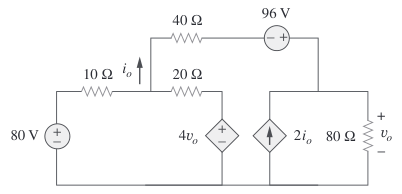
\includegraphics[width=0.5\textwidth]{./fig/fig3.30.png}
  \caption{Esquema para o Problema 19}\label{fig:fig3.30}
\end{figure}
\answer{
  \begin{align*}
    &i_0 = \frac{v_1 - (v_0 - 96)}{40} \\
    &v_0\text{:} \\
    &2i_0 + i_0 = \frac{v_0}{80} \\
    &3(\frac{v_1 - (v_0 - 96)}{40}) = \frac{v_0}{80} \\
    &7v_0 - 6v_1 = 576 \\[8pt]
    &v_1\text{:} \\
    &\frac{80 - v_1}{10} + \frac{4v_0 - v_1}{20} = i_0 \\
    &\frac{160 + 4v_0 - 3v_1}{20} = \frac{v_1 - v_0 + 96}{40} \\
    &-9v_0 + 7v_1 = 224 \\[8pt]
    &\begin{cases}
      &7v_0 - 6v_1 = 576 \\
      &-9v_0 + 7v_1 = 224 \\
    \end{cases}\\
    &v_0 = \boxed{-1075.2V} \\
    &v_1 = \boxed{-4.48V} \\
  \end{align*}
}

\newpage
\question{Determine as tensões nodais para o circuito da
Figura~\ref{fig:fig3.31}.}
\begin{figure}[H]
  \centering
  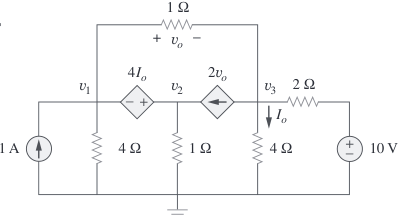
\includegraphics[width=0.5\textwidth]{./fig/fig3.31.png}
  \caption{Esquema para o Problema 20}\label{fig:fig3.31}
\end{figure}
\answer{
  \begin{align*}
    &v_2\text{:} \\
    &I_{21} = v_1 - 3v_3 \\[8pt]
    &v_1\text{:} \\
    &v_1 + 8v_3 = 4 \\[8pt]
    &v_3\text{:} \\
    &v_3 = 4v_1 - 20 \\[8pt]
    &v_1 = \frac{164}{33} = \boxed{4.97V} \\
    &v_3 = \boxed{-0.12V} \\
    &v_2 = \boxed{4.85V} \\
  \end{align*}
}

\newpage
\question{Obtenha as tensões nodais $v_1$ e $v_2$ no circuito da
Figura~\ref{fig:fig3.32}.}
\begin{figure}[H]
  \centering
  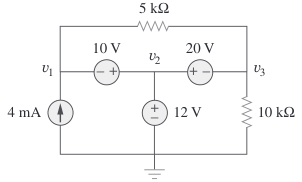
\includegraphics[width=0.5\textwidth]{./fig/fig3.32.png}
  \caption{Esquema para o Problema 21}\label{fig:fig3.32}
\end{figure}
\answer{
  \begin{align*}
    &v_2 = \boxed{12V} \\
    &v_2 - v_1 = 10 \\
    &12 - v_1 = 10 \\
    &v_1 = \boxed{2V} \\
    &v_2 - v_3 = 20 \\
    &12 - v_3 = 20 \\
    &v_3 = \boxed{-8V} \\
  \end{align*}
}

\newpage
\subsection{Análise de Malha}

Relativo a análise de malha serão feitos os problemas: 3.35, 3.37, 3.38, 3.40,
3.43, 3.44, 3.45, 3.49, 3.50, 3.52, 3.59, 3.60, 3.62, 3.63, 3.64, 3.65. Nesta
ordem.

\question{Obtenha $v_0$ no circuito da Figura~\ref{fig:fig3.5} usando análise de
malha.}
\begin{figure}[H]
  \centering
  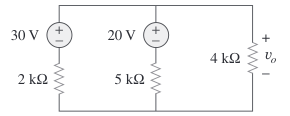
\includegraphics[width=0.5\textwidth]{./fig/fig3.5.png}
  \caption{Esquema para o Problema 22}
\end{figure}
\answer{
  \begin{align*}
    &i_1\text{:} \\
    &2i_1 - 30 + 20 + 5(i_1 - i_2) = 0 \\
    &7i_1 - 5i_2 = 10 \\[8pt]
    &i_2\text{:} \\
    &5(i_2 - i_1) - 20 + 4i_2 = 0 \\
    &-5i_1 + 9i_2 = 20 \\[8pt]
    &i_2 = 5mA \\[8pt]
    &v_0 = 4i_2 = \boxed{20V}\\
  \end{align*}
}

\newpage
\question{Usando análise de malha, determine $v_0$ no circuito da
Figura~\ref{fig:fig3.8}.}
\begin{figure}[H]
  \centering
  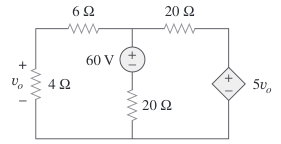
\includegraphics[width=0.5\textwidth]{./fig/fig3.8.png}
  \caption{Esquema para o Problema 23}
\end{figure}
\answer{
  \begin{align*}
    &i_1\text{:} \\
    &4i_1 + 6i_1 + 60 + 20(i_1 - i_2) = 0 \\
    &3i_1 - 2i_2 = -6 \\[8pt]
    &i_2\text{:} \\
    &20(i_2 - i_1) - 60 + 20i_2 + 5v_0 = 0 \\
    &-2i_1 + 2i_2 = 3 \\[8pt]
    &i_1 = -3A \\[8pt]
    &v_0 = -4i_1 = \boxed{12V}\\
  \end{align*}
}

\newpage
\question{Aplique análise de malhas ao circuito da Figura~\ref{fig:fig3.38} e
obtenha $I_0$.}
\begin{figure}[H]
  \centering
  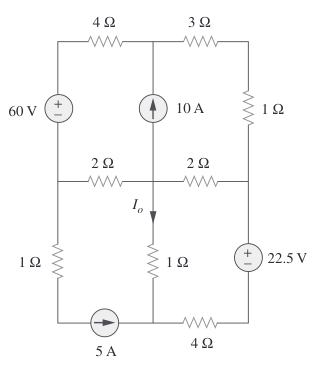
\includegraphics[width=0.5\textwidth]{./fig/fig3.38.png}
  \caption{Esquema para o Problema 24}\label{fig:fig3.38}
\end{figure}
\answer{
  \begin{align*}
    &i_1\text{:} \\
    &i_1 = -5A \\[8pt]
    &i_2\text{:} \\
    &1(i_2 - i_1) + 2(i_2 - i_4) + 22.5 + 4_i2 = 0 \\
    &7i_2 - 2i_4 = -27.5 \\[8pt]
    &i_3\text{:} \\
    &-60 + 4i_3 + 4v_{34} + 2(i_3 - i_1) = 0\\
    &6i_3 + v_{34} = 50 \\[8pt]
    &i_4\text{:} \\
    &-v_{34} + 4i_4 + 2(i_4 - i_2) = 0 \\
    &-2i_2 + 6i_4 - v_{34} = 0 \\[8pt]
    &-i_3 + i_4 = 10 \\[8pt]
    &\begin{cases}
      &7i_2 - 2i_4 = -27.5 \\
      &6i_3 + v_{34} = 50 \\
      &-2i_2 + 6i_4 - v_{34} = 0 \\
      &-i_3 + i_4 = 10 \\
    \end{cases}\\
    &i_2 = 1.375A \\
    &i_0 = i_1 - i_2 = \boxed{-6.375A} \\
  \end{align*}
}

\newpage
\question{Para o circuito em ponte da Figura~\ref{fig:fig3.40}, determine $i_0$
usando análise de malhas.}
\begin{figure}[H]
  \centering
  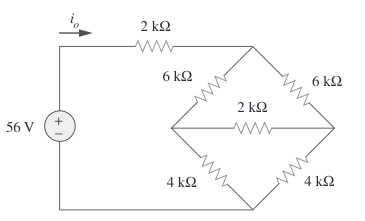
\includegraphics[width=0.5\textwidth]{./fig/fig3.40.png}
  \caption{Esquema para o Problema 25}\label{fig:fig3.40}
\end{figure}
\answer{
  \begin{align*}
    &i_1\text{:} \\
    &-56 + 2i_1 + 6(i_1 - i_2) + 4(i_1 - i_3) = 0\\
    &12i_1 - 6i_2 - 4i_3 = 56 \\[8pt]
    &i_2\text{:} \\
    &6(i_2 - i_1) + 6i_2 + 2(i_2 - i_3) = 0 \\
    &-6i_1 + 14i_2 - 2i_3 = 0 \\[8pt]
    &i_3\text{:} \\
    &4(i_3 - i_1) + 2(i_3 - i_2) + 4i_3 = 0\\
    &-4i_1 - 2i_2 + 10i_3 = 0 \\[8pt]
    &\begin{cases}
      &12i_1 - 6i_2 - 4i_3 = 56 \\
      &-6i_1 + 14i_2 - 2i_3 = 0 \\
      &-4i_1 - 2i_2 + 10i_3 = 0 \\
    \end{cases}\\
    &i_3 = 4mA \\
    &i_2 = 4mA \\
    &i_1 = 8mA \\
    &i_0 = i_1 = \boxed{8mA} \\
  \end{align*}
}

\newpage
\question{Use a análise de malhas para determinar $v_{ab}$ e $i_0$ no circui- to da
Figura~\ref{fig:fig3.43}.}
\begin{figure}[H]
  \centering
  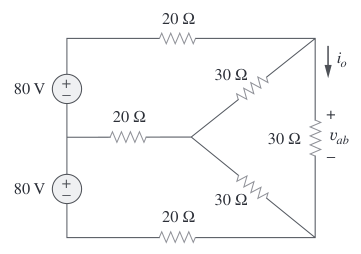
\includegraphics[width=0.5\textwidth]{./fig/fig3.43.png}
  \caption{Esquema para o Problema 26}\label{fig:fig3.43}
\end{figure}
\answer{
  \begin{align*}
    &v_{ab} = i_0 \cdot 30 \\
    &i_0 = i_3 \\
    &i_1\text{:} \\
    &-80 + 20i_1 + 30(i_1 - i_3) + 20(i_1 - i_2) = 0\\
    &70i_1 - 20i_2 - 30i_3 = 80 \\[8pt]
    &i_2\text{:} \\
    &-80 + 20(i_2 - i_1) + 30(i_2 - i_3) + 20i_2 = 0 \\
    &-20i_1 + 70i_2 - 30i_3 = 80 \\[8pt]
    &i_3\text{:} \\
    &30(i_3 - i_1) + 30i_3 + 30(i_3 - i_2) = 0\\
    &-30i_1 - 30i_2 + 90i_3 = 0 \\[8pt]
    &\begin{cases}
      &70i_1 - 20i_2 - 30i_3 = 80 \\
      &-20i_1 + 70i_2 - 30i_3 = 80 \\
      &-30i_1 - 30i_2 + 90i_3 = 0 \\
    \end{cases}\\
    &i_1 = 2.667A \\
    &i_2 = 2.667A \\
    &i_3 = 1.778A \\
    &i_0 = i_3 = \boxed{1.778A} \\
    &v_{ab} = i_0 \cdot 30 = \boxed{53.34V} \\
  \end{align*}
}

\newpage
\question{Use análise de malhas para determinar $i_0$ no circuito da
Figura~\ref{fig:fig3.44}.}
\begin{figure}[H]
  \centering
  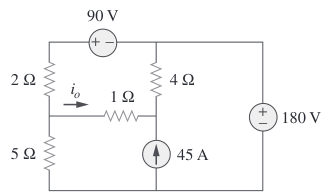
\includegraphics[width=0.5\textwidth]{./fig/fig3.44.png}
  \caption{Esquema para o Problema 27}\label{fig:fig3.44}
\end{figure}
\answer{
  \begin{align*}
    &i_1\text{:} \\
    &5i_1 + 1(i_1 - i_2) + v_{13} = 0\\
    &6i_1 - i_2 + v_{13} = 0 \\[8pt]
    &i_2\text{:} \\
    &2i_2 + 90 + 4(i_2 - i_3) + 1(i_2 - i_1) = 0 \\
    &-i_1 + 7i_2 - 4i_3 = -90 \\[8pt]
    &i_3\text{:} \\
    &-v_{13} + 4(i_3 - i_2) + 80 = 0\\
    &-4i_2 + 4i_3 - v_{13} = -80 \\[8pt]
    &i_{13}\text{:} \\
    &45 = i_3 - i_1\\[8pt]
    &\begin{cases}
      &6i_1 - i_2 + v_{13} = 0 \\
      &-i_1 + 7i_2 - 4i_3 = -90 \\
      &-4i_2 + 4i_3 - v_{13} = -80 \\
      &i_1 + i_3 = 45\\
    \end{cases}\\
    &v_{13} = 256V \\
    &i_1 = -46A \\
    &i_2 = -20A \\
    &i_3 = -1A \\
    &i_0 = i_1 - i_2 = \boxed{-26A} \\
  \end{align*}
}

\newpage
\question{Determine a corrente $i$ no circuito da Figura~\ref{fig:fig3.45}.}
\begin{figure}[H]
  \centering
  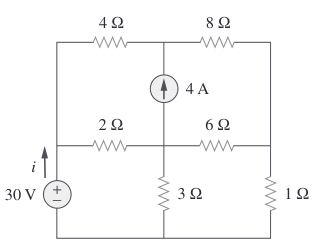
\includegraphics[width=0.5\textwidth]{./fig/fig3.45.png}
  \caption{Esquema para o Problema 28}\label{fig:fig3.45}
\end{figure}
\answer{
  \begin{align*}
    &i_3 - i_4 = 4\\[8pt]
    &i_1\text{:} \\
    &-30 + 2(i_1 - i_4) + 3(i_1 - i_2) = 0\\
    &5i_1 - 3i_2 - 2i_4  = 30 \\[8pt]
    &i_2\text{:} \\
    &3(i_2 - i_1) + 6(i_2 - i_3) + i_2 = 0 \\
    &-3i_1 + 10i_2 - 6i_3 = 0 \\[8pt]
    &i_3\text{:} \\
    &-v_{34} + 8i_3 + 6(i_3 - i_2) = 0\\
    &-6i_2 + 14i_3 - v_{34} = 0 \\[8pt]
    &i_4\text{:} \\
    &v_{34} + 2(i_4 - i_1) + 4i_4 = 0\\
    &-2i_1 + 6i_4 + v_{34} = 0 \\[8pt]
    &\begin{cases}
      &5i_1 - 3i_2 - 2i_4  = 30 \\
      &-3i_1 + 10i_2 - 6i_3 = 0 \\
      &-6i_2 + 14i_3 - v_{34} = 0 \\
      &-2i_1 + 6i_4 + v_{34} = 0 \\
    \end{cases}\\
    &i_1 = 8.561A \\
    &i = i_1 = \boxed{8.561A} \\
  \end{align*}
}

\newpage
\question{Determine $v_0$ e $i_0$ no circuito da Figura~\ref{fig:fig3.49}.}
\begin{figure}[H]
  \centering
  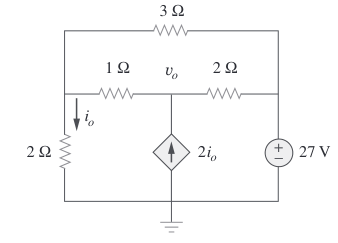
\includegraphics[width=0.5\textwidth]{./fig/fig3.49.png}
  \caption{Esquema para o Problema 29}\label{fig:fig3.49}
\end{figure}
\answer{
  \begin{align*}
    &i_0 = i_1 \\
    &i_{12}\text{:} \\
    &2i_1 - 27 + 2(i_2 - i_3) + 1(i_1 - i_3) = 0\\
    &3i_1 + 2i_2 - 3i_3  = 27 \\[8pt]
    &i_3\text{:} \\
    &3i_3 + 1(i_3 - i_1) + 2(i_3 - i_2) = 0 \\
    &-i_1 - 2i_2 + 6i_3 = 0 \\[8pt]
    &i_{12}\text{:} \\
    &i_1 - i_2 = 2i_0 \\
    &i_1 - i_2 = 2i_1 \\
    &i_1 + i_2 = 0 \\[8pt]
    &\begin{cases}
      &3i_1 + 2i_2 - 3i_3  = 27 \\
      &-i_1 - 2i_2 + 6i_3 = 0 \\
      &i_1 + i_2 = 0 \\
    \end{cases}\\
    &i_1 = 18A \\
    &i_2 = -18A \\
    &i_3 = -3A \\
    &i_0 = i_1 = \boxed{18A} \\[8pt]
    &i_3 - i_2 = \frac{v_0 - 27}{2} \\
    &v_0 = \boxed{57V} \\
  \end{align*}
}

\newpage
\question{Use a análise de malhas para determinar a corrente $i_0$ no circuito
da Figura~\ref{fig:fig3.50}.}
\begin{figure}[H]
  \centering
  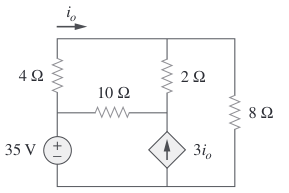
\includegraphics[width=0.5\textwidth]{./fig/fig3.50.png}
  \caption{Esquema para o Problema 30}\label{fig:fig3.50}
\end{figure}
\answer{
  \begin{align*}
    &i_0 = i_3 \\
    &i_1\text{:} \\
    &-35 + 10(i_1 - i_3) + v_0 = 0\\
    &10i_1 - 10i_3 + v_0 = 35 \\[8pt]
    &i_2\text{:} \\
    &-v_0 + 2(i_2 - i_3) + 8i_2 = 0 \\
    &10i_2 - 2i_3 - v_0 = 0 \\[8pt]
    &i_3\text{:} \\
    &4i_3 + 2(i_3 - i_2) + 10(i_3 - i_1) = 0 \\
    &-10i_1 - 2i_2 + 16i_3= 0 \\[8pt]
    &v_0\text{:} \\
    &i_2 - i_1 = 3i_0 \\
    &i_2 - i_1 = 3i_3 \\
    &i_1 - i_2 + 3i_3 = 0 \\[8pt]
    &\begin{cases}
    &10i_1 - 10i_3 + v_0 = 35 \\
    &10i_2 - 2i_3 - v_0 = 0 \\
    &-10i_1 - 2i_2 + 16i_3= 0 \\
    &i_1 - i_2 + 3i_3 = 0 \\
    \end{cases}\\
    &i_1 = 0.8413A \\
    &i_2 = 3.8702A \\
    &i_3 = 1.0096A \\
    &v_0 = 36.6827A \\
    &i_0 = i_3 = \boxed{1.0096A} \\
  \end{align*}
}

\newpage
\question{Use a análise de malhas para determinar $i_1$, $i_2$ e $i_3$ no
circuito da Figura~\ref{fig:fig3.52}.}
\begin{figure}[H]
  \centering
  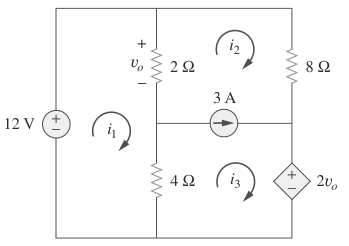
\includegraphics[width=0.5\textwidth]{./fig/fig3.52.png}
  \caption{Esquema para o Problema 31}\label{fig:fig3.52}
\end{figure}
\answer{
  \begin{align*}
    &v_0 = 2(i_2 - i_1) \\
    &i_1\text{:} \\
    &-12 + 2(i_1 - i_2) + 4(i_1 - i_3) = 0\\
    &6i_1 - 2i_2 - 4i_3 = 12 \\[8pt]
    &i_{23}\text{:} \\
    &2(i_2 - i_1) + 8i_2 + 2v_0 + 4(i_3 - i_1) = 0 \\
    &-6i_1 + 10i_2 + 4i_3 + 2v_0 = 0 \\
    &-2i_1 + 6i_2 + 4i_3 = 0 \\[8pt]
    &i_{23}\text{:} \\
    &i_2 - i_3 = -3 \\[8pt]
    &\begin{cases}
      &6i_1 - 2i_2 - 4i_3 = 12 \\[8pt]
      &-2i_1 + 6i_2 + 4i_3 = 0 \\[8pt]
      &i_2 - i_3 = -3 \\[8pt]
    \end{cases}\\
    &i_1 = 3.5A \\
    &i_2 = -0.5A \\
    &i_3 = 2.5A \\
  \end{align*}
}

\newpage
\question{Usando a análise de malha, determine $v_0$ e $i_0$ no circuito da
Figura~\ref{fig:fig3.30}.}
\begin{figure}[H]
  \centering
  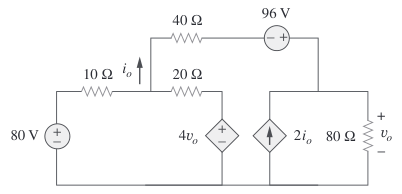
\includegraphics[width=0.5\textwidth]{./fig/fig3.30.png}
  \caption{Esquema para o Problema 32}
\end{figure}
\answer{
  \begin{align*}
    &i_{1}\text{:} \\
    &-80 + 10i_1 + 20(i_1 - i_2) + 4v_0 = 0 \\
    &30i_1 - 20i_2 + 4v_0 = 80 \\[8pt]
    &i_{23}\text{:} \\
    &-4v_0 + 20(i_2 - i_1) + 40i_2 - 96 + 80i_3 = 0 \\
    &-20i_1 + 60i_2 + 80i_3 - 4v_0 = 96 \\[8pt]
    &i_{23}\text{:} \\
    &i_2 + 2i_0 = i_3 \\
    &i_2 + 2i_2 = i_3 \\
    &3i_2 - i_3 = 0 \\[8pt]
    &\begin{cases}
      &30i_1 - 20i_2 + 4v_0 = 80 \\
      &-20i_1 + 60i_2 + 80i_3 - 4v_0 = 96 \\
      &3i_2 - i_3 = 0 \\
    \end{cases}\\
    &i_1 = 143.04A \\
    &i_2 = -4.48A \\
    &i_3 = -13.44A \\
    &i_0 = i_2 = \boxed{-4.48A} \\
    &v_0 = 80i_3 = \boxed{-1.0752kV} \\
  \end{align*}
}

\newpage
\question{Calcule a potência dissipada em cada resistor no circuito da
Figura~\ref{fig:fig3.60}.}
\begin{figure}[H]
  \centering
  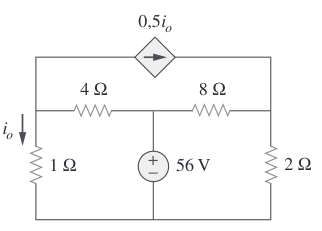
\includegraphics[width=0.5\textwidth]{./fig/fig3.60.png}
  \caption{Esquema para o Problema 33}\label{fig:fig3.60}
\end{figure}
\answer{
  \begin{align*}
    &i_3\text{:} \\
    &i_3 = 0.5i_0 \\
    &i_0 = -i_1 \\
    &i_1 = -2i_3 \\[8pt]
    &i_1\text{:} \\
    &i_1 + 4(i_1 - i_3) + 56 = 0 \\
    &5i_1 - 4i_3 = -56 \\
    &5(-2i_3) - 4i_3 = -56 \\
    &-14i_3 = -56 \\
    &i_3 = 4A \\
    &i_1 = -8A \\[8pt]
    &i_2\text{:} \\
    &-56 + 8(i_2 - i_3) + 2i_2 = 0 \\
    &i_2 = 8.8A \\[16pt]
    &P = I^2 R \\
    &P_1 = \boxed{64W} \\
    &P_4 = \boxed{1128.96W} \\
    &P_8 = \boxed{184.32W} \\
    &P_2 = \boxed{154.88W} \\
  \end{align*}
}

\newpage
\question{Determine as correntes de malha $i_1$, $i_2$ e $i_3$ na rede da
Figura~\ref{fig:fig3.62}.}
\begin{figure}[H]
  \centering
  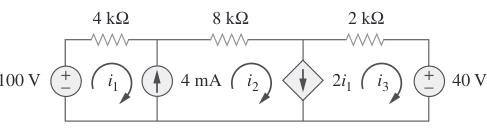
\includegraphics[width=0.5\textwidth]{./fig/fig3.62.png}
  \caption{Esquema para o Problema 34}\label{fig:fig3.62}
\end{figure}
\answer{
  \begin{align*}
    &i_{123}\text{:} \\
    &-100 + 4i_1 + 8i_2 + 2i_3 + 40 = 0 \\
    &4i_1 + 8i_2 + 2i_3 = 60 \\[8pt]
    &i_A\text{:} \\
    &i_1 + 4 = i_2 \\
    &i_1 - i_2 = -4 \\[8pt]
    &i_B\text{:} \\
    &i_2 = i_3 + 2i_1 \\
    &2i_1 - i_2 + i_3 = 0 \\[8pt]
    &\begin{cases}
      &4i_1 + 8i_2 + 2i_3 = 60 \\
      &i_1 - i_2 = -4 \\
      &2i_1 - i_2 + i_3 = 0 \\
    \end{cases}\\
    &i_1 = \boxed{2mA} \\
    &i_2 = \boxed{6mA} \\
    &i_3 = \boxed{2mA} \\
  \end{align*}
}

\newpage
\question{Determine $v_x$ e $i_x$ no circuito mostrado na
Figura~\ref{fig:fig3.63}.}
\begin{figure}[H]
  \centering
  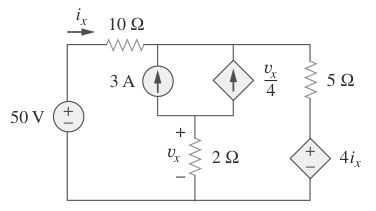
\includegraphics[width=0.5\textwidth]{./fig/fig3.63.png}
  \caption{Esquema para o Problema 35}\label{fig:fig3.63}
\end{figure}
\answer{
  \begin{align*}
    &i_x = i_1 \\
    &i_{12}\text{:} \\
    &-50 + 10i_1 + 5i_2 + 4i_x = 0 \\
    &14i_x + 5i_2 = 50 \\[8pt]
    &i_A\text{:} \\
    &i_x + 3 + \frac{v_x}{4} = i_2 \\
    &i_x - i_2 = -2 \\[8pt]
    &\begin{cases}
      &14i_x + 5i_2 = 50 \\
      &i_x - i_2 = -2 \\
    \end{cases}\\
    &i_2 = 4.105A \\
    &i_x = \boxed{2.105A} \\
    &v_x = 2(i_1 - i_2) = \boxed{-4V} \\
  \end{align*}
}

\newpage
\question{Determine $v_0$ e $i_0$ no circuito da Figura~\ref{fig:fig3.64}.}
\begin{figure}[H]
  \centering
  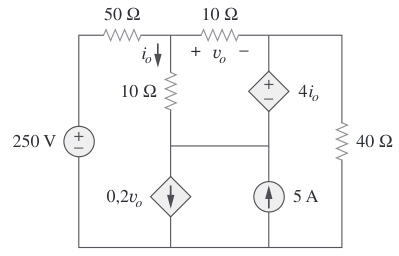
\includegraphics[width=0.5\textwidth]{./fig/fig3.64.png}
  \caption{Esquema para o Problema 36}\label{fig:fig3.64}
\end{figure}
\answer{
  \begin{align*}
    &i_2\text{:} \\
    &10(i_2 - i_1) + 10i_2 + 4i_0 = 0 \\
    &-3i_1 + 8i_2 = 0 \\[8pt]
    &i_{1234}\text{:} \\
    &-250 + 50i_1 + 10i_2 + 40i_4 = 0 \\
    &50i_1 + 10i_2 + 40i_4 = 250 \\[8pt]
    &i_{5A}\text{:} \\
    &-i_3 + i_4 = 5 \\[8pt]
    &i_{0.2v_0}\text{:} \\
    &i_1 - 2i_2 - i_3 = 0 \\[8pt]
    &\begin{cases}
      &-3i_1 + 8i_2 = 0 \\
      &50i_1 + 10i_2 + 40i_4 = 250 \\
      &-i_3 + i_4 = 5 \\
      &i_1 - 2i_2 - i_3 = 0 \\
    \end{cases}\\
    &i_1 = 0.7843A \\
    &i_2 = 0.2941A \\
    &i_3 = 0.1961A \\
    &i_4 = 5.1961A \\
    &v_0 = i_2 \cdot 10 = \boxed{2.941V} \\
    &i_0 = i_1 - i_2 = \boxed{0.4902A} \\
  \end{align*}
}

\newpage
\question{Use o \textit{MATLAB} para descobrir as correntes de malha no circuito
da Figura~\ref{fig:fig3.65}.}
\begin{figure}[H]
  \centering
  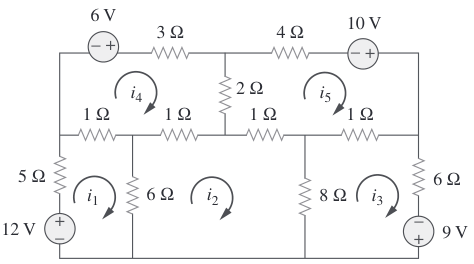
\includegraphics[width=0.5\textwidth]{./fig/fig3.65.png}
  \caption{Esquema para o Problema 37}\label{fig:fig3.65}
\end{figure}
\answer{
  \begin{align*}
    &i_1\text{:} \\
    &-12 + 5i_1 + 1(i_1 - i_4) + 6(i_1 - i_2) = 0 \\
    &12i_1 - 6i_2 - i_4 = 12 \\[8pt]
    &i_2\text{:} \\
    &6(i_2 - i_1) + 1(i_2 - i_4) + 1(i_2 - i_5) + 8(i_2 - i_3) = 0 \\
    &-6i_1 + 16i_2 - 8i_3 - i_4 - i_5 = 0 \\[8pt]
    &i_3\text{:} \\
    &8(i_3 - i_2) + 1(i_3 - i_5) + 6i_3 -9 = 0 \\
    &-8i_2 + 15i_3 - i_5 = 9 \\[8pt]
    &i_4\text{:} \\
    &-6 + 3i_4 + 2(i_4 - i_5) + 1(i_4 - i_2) + 1(i_4 - i_1) = 0 \\
    &-i_1 - i_2 + 7i_4 - 2i_5 = 6 \\[8pt]
    &i_5\text{:} \\
    &4i_5 - 10 + 1(i_5 - i_3) + 1(i_5 - i_2) + 2(i_5 - i_2) = 0 \\
    &-i_2 - i_3 - 2i_4 + 8i_5 = 10 \\[8pt]
    &\begin{cases}
    &12i_1 - 6i_2 - i_4 = 12 \\
    &-6i_1 + 16i_2 - 8i_3 - i_4 - i_5 = 0 \\
    &-8i_2 + 15i_3 - i_5 = 9 \\
    &-i_1 - i_2 + 7i_4 - 2i_5 = 6 \\
    &-i_2 - i_3 - 2i_4 + 8i_5 = 10 \\
    \end{cases}\\
    &i_1 = \boxed{2.17A} \\
    &i_2 = \boxed{1.99A} \\
    &i_3 = \boxed{1.81A} \\
    &i_4 = \boxed{2.09A} \\
    &i_4 = \boxed{2.25A} \\
  \end{align*}
}
